% !TEX root = ../ac_paper.tex

\section{Reinforcement Learning}\label{sec:rl}

%In this paper, we trained these learning algorithms with limited computation power but noticed that they easily outperform breadth-first search and often find shorter sequences of AC moves compared to the greedy search when they solve a presentation.

This section is organized as follows: in \autoref{sec:mdp}, we discuss how the problem underlying the Andrews--Curtis conjecture can be formulated as a Markov Decision Process.
In \autoref{sec:ppo}, we discuss details of a specific reinforcement learning algorithm, called the Proximal Policy Optimization algorithm, which we used to find AC trivializations of balanced presentations.
Finally, in \autoref{sec:application}, we discuss the results of our work, comparing the performance of PPO with that of the classical search algorithms studied in the previous section.

\subsection{Markov Decision Process} \label{sec:mdp}

A \textit{Markov Decision Process} (MDP) is a 5-tuple $(S, A, R, P, \rho)$ where
\begin{itemize}
	\item $S$ is the space of states,
	\item $A$ is the set of actions, i.e. $\forall a \in A, \ a \colon S \to S$,
	\item $R \colon S \times A \times S \to \mathbb{R}$ is the ``reward" function,
	\item $P \colon S \times A \to \mathcal{P}(S)$ is the transition probability function, and
	\item $\rho$ is the initial probability distribution of states.
\end{itemize}

The schematic picture of how these objects interact with each other is as follows. We start with a state $s_0$ sampled from the distribution $\rho$ and take an action $a_0$. This results in a state $s_1$ with probability $P(s_1 \mid s_0, a_0) $. The transition gets a ``reward" $r_0 = R(s_0, a_0, s_1)$ which quantifies the effectiveness of the action in contributing toward achieving an ultimate goal. From state $s_1$, we repeat this process, obtaining a trajectory of states
\[
\tau = \left( s_0, a_0, s_1, a_1, \dots \right).
\]
The goal of this process is to maximize the cumulative return,
\[
R(\tau) = \sum\limits_{t=0}^{T} \gamma^t R(s_t, a_t, s_{t+1}).
\]
Here, $T$ is the length of the trajectory, known as the ``horizon length'' and $\gamma \in \left(0, 1 \right)$ is the ``discount factor'' that assigns smaller weights to the reward values obtained farther in the future.

For a given problem at hand, we may not \textit{a priori} know the actions $\{a_t\}$ and states $\{s_{t+1}\}$ that maximize the return. Deep reinforcement learning presents a solution to this problem: we train a neural network that learns a map from states to actions with the objective of maximizing the cumulative return. More precisely, we learn a map called the ``policy" function $\pi \colon S \to \mathcal{P}(A)$ that assigns to each state a probability distribution over actions. At time step $t$, an action $a_t \sim \pi(\cdot \mid s_t)$ is sampled that gives the next state $s_{t+1}$.\footnote{
In general, we need to specify the probability transition function $P(\cdot \mid s_t, a_t)$  from which the next state would be sampled. In this paper, we take this probability distribution to be a delta function centered at a single state, which we write as $a_t(s_t)$.}
In the next subsection we discuss the specific algorithm and the objective function that we used in our study.

\subsection{Proximal Policy Optimization} \label{sec:ppo}

The goal of our optimization process is to find a policy that maximizes the cumulative return. The most naive way to achieve this goal is through an algorithm known as ``vanilla policy gradient.''
We perform gradient updates guided by the expected return $J(\pi_\theta) \equiv \mathbb{E}_{\tau \sim \pi_\theta} R(\tau)$, where the expectation is over a set of trajectories consisting of states and actions sampled according to our current policy,
\[
\theta_{k+1} = \theta_k + \nabla_\theta J(\pi_\theta).
\]

It turns out that this update depends on the gradient of the logarithm of the policy function itself and an ``advantage function'' \( A^\pi (s, a) \) which quantifies the relative benefit of taking action \( a \) in state \( s \) under policy \( \pi \) \cite{SpinningUp2018}.\footnote{
Mathematically, the advantage function is the difference between ``on-policy action-value function" $Q^{\pi}(s, a) = \mathbb{E}_{\tau \sim \pi_\theta} [R(\tau) \mid s_0 = s, a_0 = a]$ and the ``on-policy value function", $V^{\pi}(s) = \mathbb{E}_{\tau \sim \pi_\theta} [R(\tau) \mid s_0 = s]$.
These functions give an estimate of the cumulative return given that the current state-action pair is $(s, a)$ in the case of $Q^\pi$ and the current state is $s$ in the case of $V^{\pi}$.
\label{ft:advantage}}
Explicitly,
\[
\nabla_\theta J(\pi_\theta) =
\mathbb{E}_{\tau \sim \pi_\theta} \left[ \sum\limits_{t=0}^T \nabla_\theta \log \pi_\theta (a_t \mid s_t) A^{\pi_\theta} (s_t, a_t) \right].
\]
Thus, vanilla policy gradient algorithm amounts to optimizing the objective function
\[
L^{PG} = \mathbb{E}_{\tau \sim \pi_\theta} \left[ \sum\limits_{t=0}^T \log \pi_\theta (a_t \mid s_t) A^{\pi_\theta} (s_t, a_t) \right].
\]
Although it has the advantage of being simple, this algorithm has the drawback of making excessively large updates, which can cause the updated policy to deviate significantly from the current policy.

Proximal Policy Optimization (PPO) algorithms seek to make these updates more robust by limiting the extent to which the policy \( \pi \) can change in a single update \cite{schulman2017proximal}.
PPO implements this through an objective function that includes a clipped probability ratio between the new policy \( \pi_\theta \) and the old policy \( \pi_{\text{old}} \), thus constraining the updates within a predefined range.
\[
L^{CLIP}(\theta) = \mathbb{E}_{t} \left[ \min(r_t(\theta) A_t, \text{clip}(r_t(\theta), 1 - \epsilon, 1 + \epsilon) A_t) \right]
\]

Here \( r_t(\theta) = \frac{\pi_\theta(a_t | s_t)}{\pi_{\text{old}}(a_t | s_t)} \) represents the probability ratio, and \( \epsilon \) is a small positive constant (commonly set around 0.1 or 0.2) that controls the clipping value.
The raw and the clipped ratio ensure that excessively large policy updates are curtailed, making the optimization process more stable.

The advantage function is estimated during the optimization process using the Generalized Advantage Estimation method of \cite{schulman2018highdimensional}.
This method requires an estimation of the on-policy value function (c.f. \autoref{ft:advantage}).
In PPO, the actor-critic framework is used for this purpose. We train two neural networks in parallel, where the ``actor" learns the policy $\pi_\theta$ and the ``critic" learns the value function.\footnote{
Sometimes, these neural networks are made to share their parameters, which helps in stability during training.
We experimented with shared as well as unshared parameters and observed better performance by keeping the parameters independent.}
The value loss $L^V$ is the mean squared error between the values for a state as estimated by the critic network before and after a gradient update.
Lastly, PPO adds entropy $S$ of the action-space distribution to the full loss function to prevent premature convergence to a suboptimal policy. The full loss function is as follows,
\[
L = \mathbb{E}_{t} \left[ L^{CLIP}(\theta) - c_1 L^{V}(\phi) + c_2 S(\pi_\theta)(s_t) \right]
\]
where $c_1$ and $c_2$ are tunable hyperparameters.

In policy gradient algorithms such as PPO, we alternate between collecting data through the current policy in the ``rollout phase" and updating the policy weights through gradient descent in the ``optimization phase". There are various hyperparameters associated to these phases, which we briefly describe now. The rollout phase involves generating multiple trajectories of the underlying Markov Decision Process in parallel using the current policy function.
The hyperparameters of this phase include the number of parallel actors $N$, the rollout length $T'$, i.e. the number of steps each actor takes, the discount factor $\gamma$ (c.f. \autoref{sec:mdp}) and a bootstrapping hyperparameter of Generalized Advantage Estimation $\lambda_{\text{GAE}}$. The dataset of $N \times T'$ examples collected in this phase is then used to update the policy. In each epoch, the dataset is shuffled and split into mini-batches before performing gradient descent.
In addition to the optimizer hyperparameters (such as learning rate schedule), the number of epochs and the size of mini-batches are hyperparameters of the optimization process.
Further details of hyperparameters are summarized in  \autoref{app:hyperparameters}.

\subsection{Application to the Andrews--Curtis Conjecture}\label{sec:application}

The set of all balanced presentations of the trivial group with a fixed number of generators and the set of AC transformations play the roles of sets $S$ and $A$, respectively. (Recall notations introduced in \autoref{sec:mdp}). Once we choose a reward function $R$ and an initial state distribution $\rho$, we may use the Proximal Policy Optimization algorithm to learn the policy function $\pi$. We tested a few different reward functions in our experiments, observing that the following candidate led to the best performance and stability in training.
\[
R(s_{t}, a_{t}, s_{t+1}) =
\begin{cases}
	-\min(10, \ \length(s_{t+1})) & \text{if length}(s_{t+1}) > 2, \\
	\hfil 1000 & \text{otherwise.}
\end{cases}
\]
Here, $\length(s_{t+1})$ is the length of the presentation at timestep $t+1$. The reward function assigns $-\min(10, \length(s_{t+1}))$ to a non-terminal state and $1000$ to a terminal state. We found that clipping the reward to $-10$ led to less variance in gradients of the loss function with respect to weights.

We define the initial state distribution as a distribution over the presentations of the Miller--Schupp series with $n \leq 7$ and $\length(w) \leq 7$. Initially, each presentation was selected exactly once in ascending order by $n$ and $\length(w)$. Following this initial sequence, we maintained an ongoing record of presentations that were either solved or unsolved at any given time. During each rollout phase, a presentation was randomly chosen from the set of solved or unsolved presentations with probabilities of  $\frac{1}{4}$ and $\frac{3}{4}$, respectively. This method was designed to allow the policy network to refine its strategies on presentations that were already solved, potentially discovering shorter sequences of AC moves, while also tackling presentations that remained unsolved.

We also need to choose a horizon length $T$ over which the cumulative return is calculated (c.f. \autoref{sec:mdp}). In reinforcement learning, training on tasks with long horizons is usually harder than on those with short horizons. This is because in long horizon tasks it is often more difficult to figure out which actions are responsible for the eventual outcomes, a problem known as the credit assignment problem. There is also more uncertainty in the returns (high variance), which can slow down convergence and destabilize the learning process. The size of the exploration space also becomes a critical issue. With longer horizons, the agent needs to explore a more diverse set of actions to learn about long-term consequences without getting stuck in suboptimal regions. However, it does not mean that we can not train well-performing agents for long-horizon tasks; rather, it indicates that with longer horizons we may need significantly stronger computational power and extended training periods.\footnote{Another option for improving performance in long-horizon tasks is to provide good intermediate rewards; unfortunately, this is rather hard in the present context of the AC conjecture.}

The horizon length $T$ is an important hyperparameter in the context of our problem as any presentation that requires a sequence of AC moves of length greater than the horizon length will necessarily remain unsolved by PPO. On the other hand, choosing a horizon length that is too long can significantly slow down the training process. Due to the limited amount of hardware available, we mostly experimented with considerably smaller values for $T$, i.e. $T=200$ and $T=400$.  With these values, PPO could solve, respectively, $431$ and $402$ presentations out of the $1190$ Miller--Schupp presentations of the initial state distribution.\footnote{We also explored the value $T=2000$. However, we found it much slower to train due to the reasons described above. We could only solve $219$ presentations of the initial state distribution in this case. This training run had not converged, and we expect that with more computational power and extended training periods, it will be worthwhile to experiment with larger values of $T$, perhaps helping us solve even more presentations than greedy search.}
In each case, these presentations formed a subset of the presentations solved by the greedy search.

In the rest of this section, we will describe some observations made with the value $T=200$.\footnote{The complete list of hyperparameters for this experiment is summarized in \autoref{app:hyperparameters}.}
In \autoref{fig:performance} above, the performance of this experiment is compared with the results of the greedy search and the breadth-first search. While PPO consistently outperformed BFS for all values of $n$ and for all lengths of presentations, it consistently underperformed compared to the greedy search.
\footnote{
The results in this section were obtained using relatively small neural networks for both the actor and the critic networks, each consisting of two layers with 512 hidden units. It is natural to assume that increasing the size of these networks could enable a PPO agent to outperform the greedy search. However, such experiments were not performed due to computational limitations. Future work could explore this direction to assess the impact of larger network architectures.
}
In \autoref{fig:path_lengths_ppo_solved_vs_unsolved}, we plot the distribution of path lengths discovered by greedy search in the two cases of presentations that could / could not be solved by PPO. It is clear that the presentations PPO solved had, in general, smaller path lengths. In particular, all of these had greedy search path lengths less than $200$.

In \autoref{fig:path_lengths_gs_vs_ppo}, we give a scatterplot of the path lengths discovered by PPO and greedy search for all of the presentations solved by PPO. We note that in many cases, PPO found shorter paths compared to the greedy search. This is expected as PPO learns to improve its strategy during the training, discovering shorter paths for presentations it may have already solved. The scatterplot shows the shortest paths discovered by PPO for each presentation. We also note that in many cases, PPO found longer paths than greedy search. This shows that our specific run exhibits a suboptimal policy. It could perhaps be improved by performing more hyperparameter tuning on the training process.

\begin{figure}
	\centering
	\begin{subfigure}[b]{0.5\textwidth}
		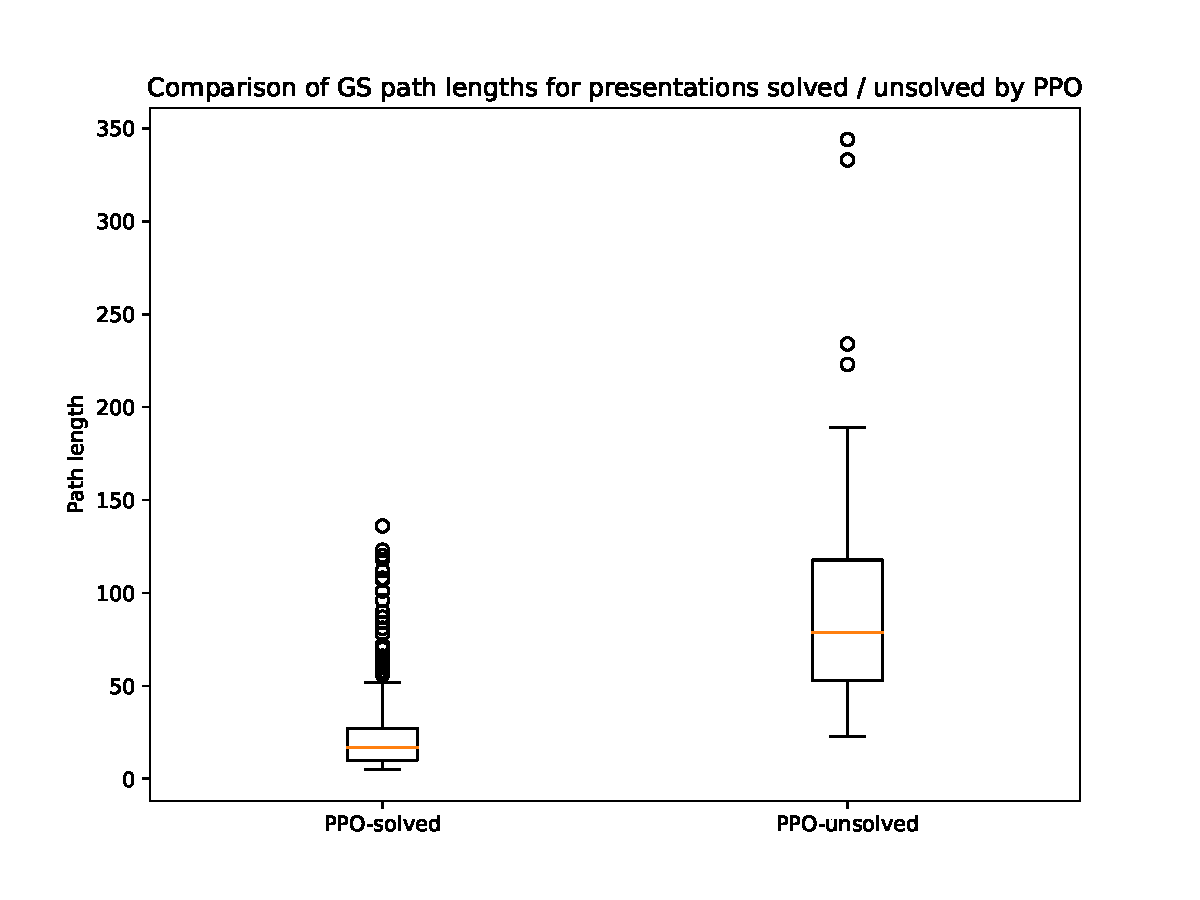
\includegraphics[width=\textwidth]{fig/path_lengths_ppo_solved_vs_unsolved.pdf}
		\caption{}
		%Distribution of path lengths discovered by greedy search for presentations solved / unsolved by Proximal Policy Optimization}
	\label{fig:path_lengths_ppo_solved_vs_unsolved}
	\end{subfigure}%
	%add desired spacing between images, e. g. ~, \quad, \qquad etc.
	%(or a blank line to force the subfigure onto a new line)
	\begin{subfigure}[b]{0.5\textwidth}
		\centering
		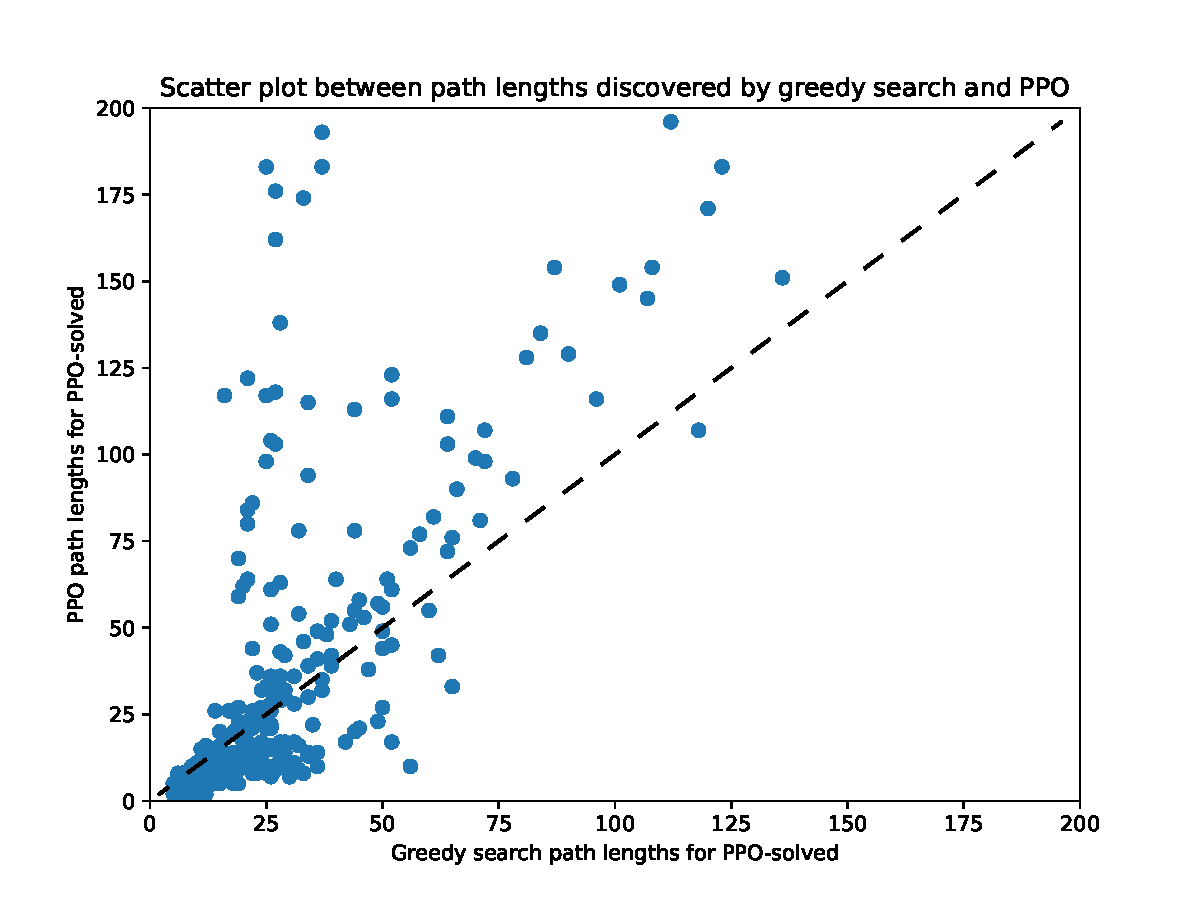
\includegraphics[width=\textwidth]{fig/path_lengths_gs_vs_ppo.pdf}
		\caption{}
		\label{fig:path_lengths_gs_vs_ppo}
	\end{subfigure}
	\caption{A comparison of path lengths discovered by the greedy search and a PPO agent. The left panel shows the distribution of lengths of AC trivialization paths discovered by the greedy search in the cases solved / unsolved by PPO. The right panel shows the scatter plot of path lengths discovered by PPO vs path lengths discovered by the greedy search.}
	\label{fig:path_lengths_gs_vs_ppo_full}
\end{figure}